\section{Additional tables and figure}
\label{app:tables}

\begin{table}[h]
\centering\small
\caption{AutoETS interval coverage and 90-day widths by stratum. Coverage is a declared secondary summary:
inclusive coverage of the repaired 0.1 to 0.9 quantiles at each horizon. The widths and the specification
counts were requested after the run, within the declared secondary calibration analysis. Widths are the
median over fits of the 90-day daily width and the median of the fit-mean width, both after clipping and
crossing repair. The last column counts fits that selected multiplicative seasonality, at each horizon.}
\label{tab:autoets}
\begin{tabular}{lrrrrrr}
\toprule
Stratum & Cov.\ $h=7$ & $h=30$ & $h=90$ & Daily width & Fit-mean width & Mult.\ fits \\
\midrule
20--99 & 0.979 & 0.978 & 0.980 & 0.79 & 0.80 & 0 \\
100--999 & 0.991 & 0.988 & 0.989 & 3.60 & 3.71 & 0 \\
1000+ & 0.991 & 0.994 & 0.995 & 49.69 & 55.99 & 6 \\
\bottomrule
\end{tabular}
\end{table}

\begin{table}[h]
\centering\small
\caption{Pooled \qs{} by day-90 stratum and horizon, declared secondary: three windows averaged within
repository, then 100 repositories per stratum weighted equally. These are stratum means; the typical
repository by stratum is given, labeled post-hoc, in Section~\ref{sec:results}.}
\label{tab:stratum}
\begin{tabular}{llrrrrr}
\toprule
Stratum & $h$ & Chronos-2 & TimesFM 3 & TimesFM 2.5 & \lm{} & \aets{} \\
\midrule
20-99 & 7 & 0.077 & 0.077 & 0.079 & 0.075 & 0.148 \\
20-99 & 30 & 0.084 & 0.084 & 0.085 & 0.082 & 0.162 \\
20-99 & 90 & 0.086 & 0.101 & 0.088 & 0.083 & 0.189 \\
100-999 & 7 & 0.217 & 0.219 & 0.226 & 0.228 & 0.542 \\
100-999 & 30 & 0.217 & 0.215 & 0.221 & 0.217 & 0.703 \\
100-999 & 90 & 0.233 & 0.231 & 0.235 & 0.236 & 0.967 \\
1000+ & 7 & 2.798 & 2.432 & 2.470 & 3.200 & 5.609 \\
1000+ & 30 & 3.134 & 2.929 & 2.923 & 3.531 & 8.950 \\
1000+ & 90 & 3.966 & 3.874 & 3.930 & 4.270 & 23.301 \\
\bottomrule
\end{tabular}
\end{table}

\begin{table}[h]
\centering\small
\caption{Inclusive 80 percent coverage of the repaired 0.1 to 0.9 quantiles, averaged within repository and
then over 300 repositories, declared secondary.}
\label{tab:calibration}
\begin{tabular}{lrrr}
\toprule
Model & $h=7$ & $h=30$ & $h=90$ \\
\midrule
chronos2 & 0.832 & 0.824 & 0.837 \\
timesfm3 & 0.880 & 0.910 & 0.889 \\
timesfm2p5 & 0.924 & 0.906 & 0.918 \\
local\_mean\_28 & 0.955 & 0.945 & 0.941 \\
autoets\_weekly & 0.987 & 0.986 & 0.988 \\
\bottomrule
\end{tabular}
\end{table}

\begin{table}[h]
\centering\small
\caption{The declared scale review against \lm{}. The top-five share divides the five largest positive
repository gains (reference minus model) by all positive gains. Skill, $1 - \text{model}/\text{reference}$,
is undefined where the reference's loss is zero. The leave-one-out range is the mean gain with each
repository removed in turn.}
\label{tab:scale}
\begin{tabular}{llrrc}
\toprule
Model & $h$ & Top-five share of positive gain & Skill defined (of 300) & Leave-one-out mean gain \\
\midrule
Chronos-2 & 7 & 0.902 & 209 & [0.060, 0.152] \\
Chronos-2 & 30 & 0.910 & 239 & [0.074, 0.134] \\
Chronos-2 & 90 & 0.892 & 259 & [0.068, 0.105] \\
TimesFM 3 & 7 & 0.932 & 209 & [0.066, 0.280] \\
TimesFM 3 & 30 & 0.929 & 239 & [0.083, 0.203] \\
TimesFM 3 & 90 & 0.895 & 259 & [0.064, 0.133] \\
TimesFM 2.5 & 7 & 0.943 & 209 & [0.049, 0.265] \\
TimesFM 2.5 & 30 & 0.943 & 239 & [0.073, 0.203] \\
TimesFM 2.5 & 90 & 0.885 & 259 & [0.046, 0.120] \\
\bottomrule
\end{tabular}
\end{table}

\begin{figure}[h]
\centering
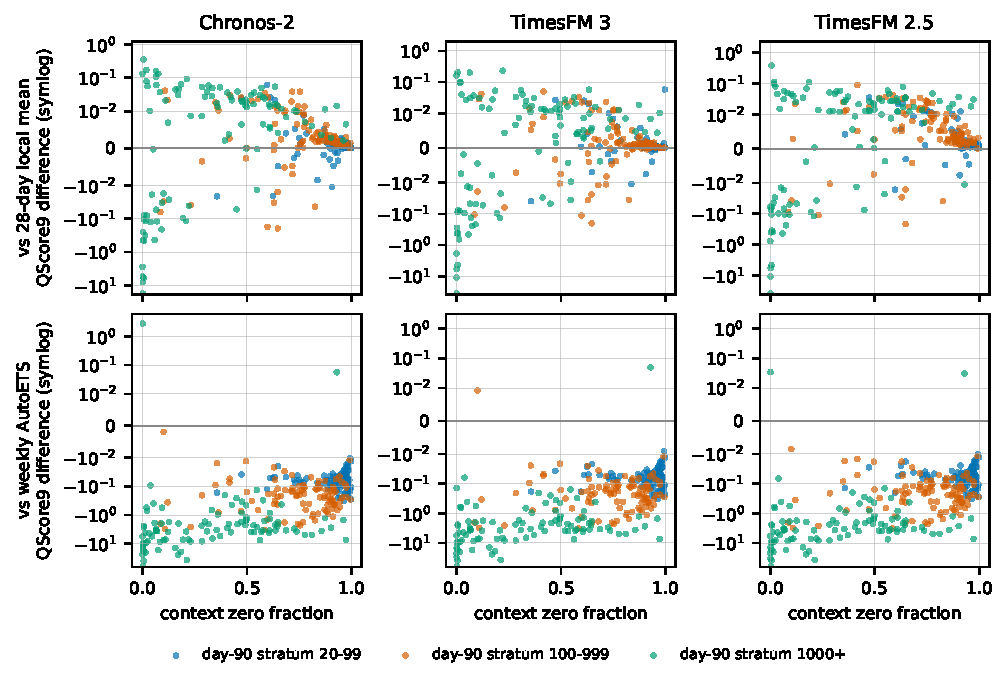
\includegraphics[width=\textwidth]{fig-posthoc-zero-fraction-h30}
\caption{Post-hoc. Each repository's paired difference at horizon 30 against the fraction of zero days in
its context (three windows averaged), colored by day-90 stratum, on a symmetric log scale. Top row: against
\lm{}; bottom row: against \aets{}. Against the local mean the large model gains are at low zero fractions
and the small model losses cluster at high ones; against AutoETS nearly every repository at every zero
fraction favors the model.}
\label{fig:zerofraction}
\end{figure}
